\chapter{Análisis del problema}

\section{Introducción}
En este capítulo se va a describir de forma más detallada el problema que se va a resolver con la aplicación a desarrollar. De esta forma, vamos a especificar qué es lo que 
tiene que hacer el sistema para su futuro desarrollo. El objetivo del análisis es definir, estructurar y describir los requisitos o historias de usuario para conseguir una comprensión
más precisa y detallada del problema a resolver.
\section{Historias de Usuario}
A continuación, se procederá a describir las historias de usuario que se han definido para el proyecto. 

\subsection*{Funcionalidad del usuario}

\begin{table}[H]
    \centering
    \resizebox{\textwidth}{!}{%
        \begin{tabular}{|
                >{\columncolor[HTML]{D8D8D8}}l |l|
                >{\columncolor[HTML]{D8D8D8}}l |l|l|l|}
            \hline
            \textbf{ID}                  & HU1                                      & \textbf{Nombre}       & \multicolumn{3}{l|}{\begin{tabular}[c]{@{}l@{}}Como usuario quiero registrarme en la aplicación para poder\\ comenzar a utilizar sus funcionalidades.\end{tabular}}\\ \hline
            \textbf{PH}                  & 2                                        & \textbf{Descripcion}  & \multicolumn{3}{l|}{\begin{tabular}[c]{@{}l@{}}El usuario podrá registrarse en el sistema rellenando un formulario\\ con campos como el nombre de usuario, el correo electrónico, la \\contraseña... \end{tabular}}  \\ \hline
            \textbf{Prioridad}           & Alta                                       & \textbf{Dependencias} & \begin{tabular}[c]{@{}l@{}} --- \end{tabular}                      & \cellcolor[HTML]{D8D8D8}\begin{tabular}[c]{@{}l@{}}\textbf{Requisitos Funcionales}\end{tabular} & \begin{tabular}[c]{@{}l@{}}RF 1\end{tabular} \\ \hline
            \multicolumn{3}{|l|}{\cellcolor[HTML]{D8D8D8}\textbf{Pruebas de aceptacion}} & \multicolumn{3}{l|}{\begin{tabular}[c]{@{}l@{}}1. Todos los campos rellenados por el usuario serán almacenados \\en la base de datos. \\ 2. La contraseña se almacenará cifrada para no comprometer la \\seguridad del usuario. \\ 3. Si el usuario introduce valores erróneos, se informará del campo \\en el que está el error. \\4. Si el usuario no introduce datos en los campos obligatorios, se \\informará de los campos que falten por rellenar.  \end{tabular}}                                                                                                                                                                                                                                                                                               \\ \hline
        \end{tabular}%
    }
\end{table}


\begin{table}[H]
    \centering
    \resizebox{\textwidth}{!}{%
        \begin{tabular}{|
                >{\columncolor[HTML]{D8D8D8}}l |l|
                >{\columncolor[HTML]{D8D8D8}}l |l|l|l|}
            \hline
            \textbf{ID}                                                                  & HU2                                      & \textbf{Nombre}       & \multicolumn{3}{l|}{\begin{tabular}[c]{@{}l@{}}Como usuario quiero iniciar sesión en la aplicación para \\poder acceder a sus funcionalidades.\end{tabular}}\\ \hline
            \textbf{PH}                  & 2                                        & \textbf{Descripcion}  & \multicolumn{3}{l|}{\begin{tabular}[c]{@{}l@{}}El usuario podrá iniciar sesióm en el sistema rellenando \\un formulario con campos  como el nombre de usuario \\o correo electrónico y la contraseña... \end{tabular}}  \\ \hline
            \textbf{Prioridad}           & Alta                                        & \textbf{Dependencias} & \begin{tabular}[c]{@{}l@{}} --- \end{tabular}                      & \cellcolor[HTML]{D8D8D8}\begin{tabular}[c]{@{}l@{}}\textbf{Requisitos Funcionales}\end{tabular} & \begin{tabular}[c]{@{}l@{}}RF 2\end{tabular} \\ \hline
            \multicolumn{3}{|l|}{\cellcolor[HTML]{D8D8D8}\textbf{Pruebas de aceptacion}} & \multicolumn{3}{l|}{\begin{tabular}[c]{@{}l@{}}1. Se compararán los campos rellenados por el usuario con los \\almacenados para comprobar la identidad del usuario.\\ 2. La contraseña procesará de forma cifrada para no comprometer\\ la seguridad del usuario. \\ 3. Si el usuario introduce datos incorrectos, se informará del error\\ al usuario. \end{tabular}}                                               \\ \hline
        \end{tabular}%
    }
\end{table}


\begin{table}[H]
    \centering
    \resizebox{\textwidth}{!}{%
        \begin{tabular}{|
                >{\columncolor[HTML]{D8D8D8}}l |l|
                >{\columncolor[HTML]{D8D8D8}}l |l|l|l|}
            \hline
            \textbf{ID}                  & HU3                                      & \textbf{Nombre}       & \multicolumn{3}{l|}{\begin{tabular}[c]{@{}l@{}}Como usuario quiero ver los datos personales y los logros.\end{tabular}}\\ \hline
            \textbf{PH}                  & 1                                     & \textbf{Descripcion}  & \multicolumn{3}{l|}{\begin{tabular}[c]{@{}l@{}}El usuario podrá visualizar todos los datos de su propio perfil como el nombre, \\ apellidos, imagen de perfil, correo, etc \end{tabular}}  \\ \hline
            \textbf{Prioridad}           & Media                                    & \textbf{Dependencias} & \begin{tabular}[c]{@{}l@{}} --- \end{tabular}                      & \cellcolor[HTML]{D8D8D8}\begin{tabular}[c]{@{}l@{}}\textbf{Requisitos Funcionales}\end{tabular} & \begin{tabular}[c]{@{}l@{}}RF 3\end{tabular} \\ \hline
            \multicolumn{3}{|l|}{\cellcolor[HTML]{D8D8D8}\textbf{Pruebas de aceptacion}} & \multicolumn{3}{l|}{\begin{tabular}[c]{@{}l@{}}1. Los datos mostrados al usuario en su perfil se corresponderán \\ con la información almacenada en la base de datos de dicho usuario. \end{tabular}}                                               \\ \hline
        \end{tabular}%
    }
\end{table}


\begin{table}[H]
    \centering
    \resizebox{\textwidth}{!}{%
        \begin{tabular}{|
                >{\columncolor[HTML]{D8D8D8}}l |l|
                >{\columncolor[HTML]{D8D8D8}}l |l|l|l|}
            \hline
            \textbf{ID}                  & HU4                                      & \textbf{Nombre}       & \multicolumn{3}{l|}{\begin{tabular}[c]{@{}l@{}}Como usuario quiero editar los datos de mi perfil.\end{tabular}}\\ \hline
            \textbf{PH}                  & 2                                       & \textbf{Descripcion}  & \multicolumn{3}{l|}{\begin{tabular}[c]{@{}l@{}}El usuario podrá modificar los datos de su perfil como su nombre de \\usuario, correo electrónico, contraseña, etc... \end{tabular}}  \\ \hline
            \textbf{Prioridad}           & Media                                        & \textbf{Dependencias} & \begin{tabular}[c]{@{}l@{}} HU 3 \end{tabular}                      & \cellcolor[HTML]{D8D8D8}\begin{tabular}[c]{@{}l@{}}\textbf{Requisitos Funcionales}\end{tabular} & \begin{tabular}[c]{@{}l@{}}RF 4\end{tabular} \\ \hline
            \multicolumn{3}{|l|}{\cellcolor[HTML]{D8D8D8}\textbf{Pruebas de aceptacion}} & \multicolumn{3}{l|}{\begin{tabular}[c]{@{}l@{}}1. Los datos introducidos por el usuario en los campos del formulario \\se actualizarán en la base de datos \\ 2. En caso de modificar la contraseña, esta se almacenará cifrada para \\no comprometer la seguridad del usuario. \\3. Si el usuario introduce valores erróneos, se informará del campo en \\el que está el error.\end{tabular}}                                               \\ \hline
        \end{tabular}%
    }
\end{table}


\begin{table}[H]
    \centering
    \resizebox{\textwidth}{!}{%
        \begin{tabular}{|
                >{\columncolor[HTML]{D8D8D8}}l |l|
                >{\columncolor[HTML]{D8D8D8}}l |l|l|l|}
            \hline
            \textbf{ID}                  & HU5                                      & \textbf{Nombre}       & \multicolumn{3}{l|}{\begin{tabular}[c]{@{}l@{}}Como usuario quiero ver en detalle uno de mis logros.\end{tabular}}\\ \hline
            \textbf{PH}                  & 1                                        & \textbf{Descripcion}  & \multicolumn{3}{l|}{\begin{tabular}[c]{@{}l@{}}El usuario podrá ver la información en detalle de cada uno de sus logros \end{tabular}}  \\ \hline
            \textbf{Prioridad}           & Baja                                        & \textbf{Dependencias} & \begin{tabular}[c]{@{}l@{}} HU 3 \end{tabular}                      & \cellcolor[HTML]{D8D8D8}\begin{tabular}[c]{@{}l@{}}\textbf{Requisitos Funcionales}\end{tabular} & \begin{tabular}[c]{@{}l@{}}RF 7\end{tabular} \\ \hline
            \multicolumn{3}{|l|}{\cellcolor[HTML]{D8D8D8}\textbf{Pruebas de aceptacion}} & \multicolumn{3}{l|}{\begin{tabular}[c]{@{}l@{}}1. Los datos mostrados al usuario respecto al logro corresponderán \\ con la información almacenada en la base de datos. \end{tabular}}                                               \\ \hline
        \end{tabular}%
    }
\end{table}


\begin{table}[H]
    \centering
    \resizebox{\textwidth}{!}{%
        \begin{tabular}{|
                >{\columncolor[HTML]{D8D8D8}}l |l|
                >{\columncolor[HTML]{D8D8D8}}l |l|l|l|}
            \hline
            \textbf{ID}                  & HU6                                      & \textbf{Nombre}       & \multicolumn{3}{l|}{\begin{tabular}[c]{@{}l@{}}Como usuario quiero seleccionar una lección para leer el temario.\end{tabular}}\\ \hline
            \textbf{PH}                  & 1                                        & \textbf{Descripcion}  & \multicolumn{3}{l|}{\begin{tabular}[c]{@{}l@{}}El usuario podrá hacer click en la lección que desea de la lista ubicada en la pantalla \\principal. \end{tabular}}  \\ \hline
            \textbf{Prioridad}           & Alta                                        & \textbf{Dependencias} & \begin{tabular}[c]{@{}l@{}} --- \end{tabular}                      & \cellcolor[HTML]{D8D8D8}\begin{tabular}[c]{@{}l@{}}\textbf{Requisitos Funcionales}\end{tabular} & \begin{tabular}[c]{@{}l@{}}RF 5\end{tabular} \\ \hline
            \multicolumn{3}{|l|}{\cellcolor[HTML]{D8D8D8}\textbf{Pruebas de aceptacion}} & \multicolumn{3}{l|}{\begin{tabular}[c]{@{}l@{}}1. El contenido (textos, imágenes, vídeos...) almacenado en la base de datos de\\ la lección seleccionada aparecerá en pantalla. \\ 2. No se podrá elegir una lección que esté bloqueada.\end{tabular}}                                               \\ \hline
        \end{tabular}%
    }
\end{table}


\begin{table}[H]
    \centering
    \resizebox{\textwidth}{!}{%
        \begin{tabular}{|
                >{\columncolor[HTML]{D8D8D8}}l |l|
                >{\columncolor[HTML]{D8D8D8}}l |l|l|l|}
            \hline
            \textbf{ID}                  & HU7                                      & \textbf{Nombre}       & \multicolumn{3}{l|}{\begin{tabular}[c]{@{}l@{}}Como usuario quiero empezar un test de una lección.\end{tabular}}\\ \hline
            \textbf{PH}                  & 1                                        & \textbf{Descripcion}  & \multicolumn{3}{l|}{\begin{tabular}[c]{@{}l@{}}El usuario pulsará el botón de empezar test ubicado dentro de la lección para poder \\responder a las preguntas.\end{tabular}}  \\ \hline
            \textbf{Prioridad}           & Alta                                        & \textbf{Dependencias} & \begin{tabular}[c]{@{}l@{}} --- \end{tabular}                      & \cellcolor[HTML]{D8D8D8}\begin{tabular}[c]{@{}l@{}}\textbf{Requisitos Funcionales}\end{tabular} & \begin{tabular}[c]{@{}l@{}}RF 6\end{tabular} \\ \hline
            \multicolumn{3}{|l|}{\cellcolor[HTML]{D8D8D8}\textbf{Pruebas de aceptacion}} & \multicolumn{3}{l|}{\begin{tabular}[c]{@{}l@{}}1. Las preguntas almacenadas en la base de datos de dicha lección aparecerán en orden.\end{tabular}}                                               \\ \hline
        \end{tabular}%
    }
\end{table}


\begin{table}[H]
    \centering
    \resizebox{\textwidth}{!}{%
        \begin{tabular}{|
                >{\columncolor[HTML]{D8D8D8}}l |l|
                >{\columncolor[HTML]{D8D8D8}}l |l|l|l|}
            \hline
            \textbf{ID}                  & HU8                                      & \textbf{Nombre}       & \multicolumn{3}{l|}{\begin{tabular}[c]{@{}l@{}}Como usuario quiero responder una pregunta de un test del tipo selección múltiple.\end{tabular}}\\ \hline
            \textbf{PH}                  & 1                                        & \textbf{Descripcion}  & \multicolumn{3}{l|}{\begin{tabular}[c]{@{}l@{}}El usuario podrá responder a una pregunta seleccionando más de una opción \\de la lista de posibles respuestas.\end{tabular}}  \\ \hline
            \textbf{Prioridad}           & Alta                                        & \textbf{Dependencias} & \begin{tabular}[c]{@{}l@{}} HU7 \end{tabular}                      & \cellcolor[HTML]{D8D8D8}\begin{tabular}[c]{@{}l@{}}\textbf{Requisitos Funcionales}\end{tabular} & \begin{tabular}[c]{@{}l@{}}RF 6.2\end{tabular} \\ \hline
            \multicolumn{3}{|l|}{\cellcolor[HTML]{D8D8D8}\textbf{Pruebas de aceptacion}} & \multicolumn{3}{l|}{\begin{tabular}[c]{@{}l@{}}1. La respuesta del usuario quedará registrada en el sistema para un futuro procesamiento. \\ 2. El usuario deberá seleccionar una respuesta como mínimo.\end{tabular}}                                               \\ \hline
        \end{tabular}%
    }
\end{table}


\begin{table}[H]
    \centering
    \resizebox{\textwidth}{!}{%
        \begin{tabular}{|
                >{\columncolor[HTML]{D8D8D8}}l |l|
                >{\columncolor[HTML]{D8D8D8}}l |l|l|l|}
            \hline
            \textbf{ID}                  & HU9                                      & \textbf{Nombre}       & \multicolumn{3}{l|}{\begin{tabular}[c]{@{}l@{}}Como usuario quiero responder una pregunta de un test del tipo selección única.\end{tabular}}\\ \hline
            \textbf{PH}                  & 1                                        & \textbf{Descripcion}  & \multicolumn{3}{l|}{\begin{tabular}[c]{@{}l@{}}El usuario podrá responder a una pregunta seleccionando una sola opción \\de la lista de posibles respuestas.\end{tabular}}  \\ \hline
            \textbf{Prioridad}           & Alta                                        & \textbf{Dependencias} & \begin{tabular}[c]{@{}l@{}} HU7 \end{tabular}                      & \cellcolor[HTML]{D8D8D8}\begin{tabular}[c]{@{}l@{}}\textbf{Requisitos Funcionales}\end{tabular} & \begin{tabular}[c]{@{}l@{}}RF 6.3\end{tabular} \\ \hline
            \multicolumn{3}{|l|}{\cellcolor[HTML]{D8D8D8}\textbf{Pruebas de aceptacion}} & \multicolumn{3}{l|}{\begin{tabular}[c]{@{}l@{}}1. La respuesta del usuario quedará registrada en el sistema para un futuro procesamiento.\\2. El usuario deberá seleccionar una opción obligatoriamente.\end{tabular}}                                               \\ \hline
        \end{tabular}%
    }
\end{table}


\begin{table}[H]
    \centering
    \resizebox{\textwidth}{!}{%
        \begin{tabular}{|
                >{\columncolor[HTML]{D8D8D8}}l |l|
                >{\columncolor[HTML]{D8D8D8}}l |l|l|l|}
            \hline
            \textbf{ID}                  & HU10                                     & \textbf{Nombre}       & \multicolumn{3}{l|}{\begin{tabular}[c]{@{}l@{}}Como usuario quiero responder una pregunta de un test del tipo respuesta por micrófono.\end{tabular}}\\ \hline
            \textbf{PH}                  & 8                                        & \textbf{Descripcion}  & \multicolumn{3}{l|}{\begin{tabular}[c]{@{}l@{}}El usuario podrá responder a una pregunta mediante la entrada de un sonido\\ de un instrumento externo a través del micrófono.\end{tabular}}  \\ \hline
            \textbf{Prioridad}           & Alta                                        & \textbf{Dependencias} & \begin{tabular}[c]{@{}l@{}} HU7 \end{tabular}                      & \cellcolor[HTML]{D8D8D8}\begin{tabular}[c]{@{}l@{}}\textbf{Requisitos Funcionales}\end{tabular} & \begin{tabular}[c]{@{}l@{}}RF 6.4\end{tabular} \\ \hline
            \multicolumn{3}{|l|}{\cellcolor[HTML]{D8D8D8}\textbf{Pruebas de aceptacion}} & \multicolumn{3}{l|}{\begin{tabular}[c]{@{}l@{}}1. La respuesta del usuario quedará registrada en el sistema para un futuro procesamiento.\end{tabular}}                                               \\ \hline
        \end{tabular}%
    }
\end{table}

\begin{table}[H]
    \centering
    \resizebox{\textwidth}{!}{%
        \begin{tabular}{|
                >{\columncolor[HTML]{D8D8D8}}l |l|
                >{\columncolor[HTML]{D8D8D8}}l |l|l|l|}
            \hline



            \textbf{ID}                  & HU26                                      & \textbf{Nombre}       & \multicolumn{3}{l|}{\begin{tabular}[c]{@{}l@{}}Como usuario quiero responder una pregunta de un test del \\tipo escritura de texto.\end{tabular}}\\ \hline
            \textbf{PH}                  & 1                                        & \textbf{Descripcion}  & \multicolumn{3}{l|}{\begin{tabular}[c]{@{}l@{}}El usuario podrá responder a una pregunta escribiendo \\la respuesta en un campo de texto. \end{tabular}}  \\ \hline
            \textbf{Prioridad}           & Media                                        & \textbf{Dependencias} & \begin{tabular}[c]{@{}l@{}} HU7 \end{tabular}                      & \cellcolor[HTML]{D8D8D8}\begin{tabular}[c]{@{}l@{}}\textbf{Requisitos Funcionales}\end{tabular} & \begin{tabular}[c]{@{}l@{}}RF 6.1\end{tabular} \\ \hline
            \multicolumn{3}{|l|}{\cellcolor[HTML]{D8D8D8}\textbf{Pruebas de aceptacion}} & \multicolumn{3}{l|}{\begin{tabular}[c]{@{}l@{}}1. La respuesta del usuario quedará registrada en el sistema para\\ un futuro procesamiento.\end{tabular}}                                               \\ \hline
        \end{tabular}%
    }
\end{table}



\begin{table}[H]
    \centering
    \resizebox{\textwidth}{!}{%
        \begin{tabular}{|
                >{\columncolor[HTML]{D8D8D8}}l |l|
                >{\columncolor[HTML]{D8D8D8}}l |l|l|l|}
            \hline
            \textbf{ID}                  & HU11                                      & \textbf{Nombre}       & \multicolumn{3}{l|}{\begin{tabular}[c]{@{}l@{}}Como usuario quiero ver el resultado de un test.\end{tabular}}\\ \hline
            \textbf{PH}                  & 2                                        & \textbf{Descripcion}  & \multicolumn{3}{l|}{\begin{tabular}[c]{@{}l@{}}El usuario podrá visualizar el resultado del test una vez finalizado.\end{tabular}}  \\ \hline
            \textbf{Prioridad}           & Media                                        & \textbf{Dependencias} & \begin{tabular}[c]{@{}l@{}} HU7, HU8, HU9, HU10, HU26 \end{tabular}                      & \cellcolor[HTML]{D8D8D8}\begin{tabular}[c]{@{}l@{}}\textbf{Requisitos Funcionales}\end{tabular} & \begin{tabular}[c]{@{}l@{}}RF 6\end{tabular} \\ \hline
            \multicolumn{3}{|l|}{\cellcolor[HTML]{D8D8D8}\textbf{Pruebas de aceptacion}} & \multicolumn{3}{l|}{\begin{tabular}[c]{@{}l@{}}1. El resultado del test será almacenado en la base de datos. \\ 2. La puntuación mostrada en pantalla corresponderá a las\\ preguntas acertadas en dicho test. \end{tabular}}                                               \\ \hline
        \end{tabular}%
    }
\end{table}


\begin{table}[H]
    \centering
    \resizebox{\textwidth}{!}{%
        \begin{tabular}{|
                >{\columncolor[HTML]{D8D8D8}}l |l|
                >{\columncolor[HTML]{D8D8D8}}l |l|l|l|}
            \hline
            \textbf{ID}                  & HU12                                      & \textbf{Nombre}       & \multicolumn{3}{l|}{\begin{tabular}[c]{@{}l@{}}Como usuario quiero ver la lista de mis logros obtenidos.\end{tabular}}\\ \hline
            \textbf{PH}                  & 0.5                                        & \textbf{Descripcion}  & \multicolumn{3}{l|}{\begin{tabular}[c]{@{}l@{}}El usuario podrá visualizar la lista de logros conseguidos durante su progreso. \end{tabular}}  \\ \hline
            \textbf{Prioridad}           & Media                                        & \textbf{Dependencias} & \begin{tabular}[c]{@{}l@{}} --- \end{tabular}                      & \cellcolor[HTML]{D8D8D8}\begin{tabular}[c]{@{}l@{}}\textbf{Requisitos Funcionales}\end{tabular} & \begin{tabular}[c]{@{}l@{}}RF 22\end{tabular} \\ \hline
            \multicolumn{3}{|l|}{\cellcolor[HTML]{D8D8D8}\textbf{Pruebas de aceptacion}} & \multicolumn{3}{l|}{\begin{tabular}[c]{@{}l@{}}1. La lista mostrará solamente los logros que el usuario tenga asociados por haberlos obtenido. \end{tabular}}                                               \\ \hline
        \end{tabular}%
    }
\end{table}


\begin{table}[H]
    \centering
    \resizebox{\textwidth}{!}{%
        \begin{tabular}{|
                >{\columncolor[HTML]{D8D8D8}}l |l|
                >{\columncolor[HTML]{D8D8D8}}l |l|l|l|}
            \hline
            \textbf{ID}                  & HU13                                      & \textbf{Nombre}       & \multicolumn{3}{l|}{\begin{tabular}[c]{@{}l@{}}Como usuario quiero ver mi progreso en las lecciones.\end{tabular}}\\ \hline
            \textbf{PH}                  & 2                                        & \textbf{Descripcion}  & \multicolumn{3}{l|}{\begin{tabular}[c]{@{}l@{}}El usuario podrá ver su progreso en cada lección, los resultados de cada test\\ y los puntos que le faltan para completar la lección.\end{tabular}}  \\ \hline
            \textbf{Prioridad}           & Media                                        & \textbf{Dependencias} & \begin{tabular}[c]{@{}l@{}} HU6 \end{tabular}                      & \cellcolor[HTML]{D8D8D8}\begin{tabular}[c]{@{}l@{}}\textbf{Requisitos Funcionales}\end{tabular} & \begin{tabular}[c]{@{}l@{}}RF 1\end{tabular} \\ \hline
            \multicolumn{3}{|l|}{\cellcolor[HTML]{D8D8D8}\textbf{Pruebas de aceptacion}} & \multicolumn{3}{l|}{\begin{tabular}[c]{@{}l@{}}1. Se mostrarán los datos relacionados con el progreso del usuario de la lección\\ correspondiente. \end{tabular}}                                               \\ \hline
        \end{tabular}%
    }
\end{table}

\subsection*{Gestión de lecciones y tests}

\begin{table}[H]
    \centering
    \resizebox{\textwidth}{!}{%
        \begin{tabular}{|
                >{\columncolor[HTML]{D8D8D8}}l |l|
                >{\columncolor[HTML]{D8D8D8}}l |l|l|l|}
            \hline
            \textbf{ID}                  & HU14                                      & \textbf{Nombre}       & \multicolumn{3}{l|}{\begin{tabular}[c]{@{}l@{}}Como profesor y administrador quiero crear una lección.\end{tabular}}\\ \hline
            \textbf{PH}                  & 1                                        & \textbf{Descripcion}  & \multicolumn{3}{l|}{\begin{tabular}[c]{@{}l@{}}El profesor podrá crear una lección, añadiendo el texto y el contenido multimedia \\ que desee. \end{tabular}}  \\ \hline
            \textbf{Prioridad}           & Media                                        & \textbf{Dependencias} & \begin{tabular}[c]{@{}l@{}} HU28 \end{tabular}                      & \cellcolor[HTML]{D8D8D8}\begin{tabular}[c]{@{}l@{}}\textbf{Requisitos Funcionales}\end{tabular} & \begin{tabular}[c]{@{}l@{}}RF 11\end{tabular} \\ \hline
            \multicolumn{3}{|l|}{\cellcolor[HTML]{D8D8D8}\textbf{Pruebas de aceptacion}} & \multicolumn{3}{l|}{\begin{tabular}[c]{@{}l@{}}1. Todos los campos rellenados por el profesor serán almacenados en la base de datos.\\ 2. Si el usuario introduce valores erróneos, se informará del campo en el que está\\ el error. \\3. Si el usuario no introduce datos en los campos obligatorios, se informará de los \\campos que falten por rellenar. \end{tabular}}                                               \\ \hline
        \end{tabular}%
    }
\end{table}


\begin{table}[H]
    \centering
    \resizebox{\textwidth}{!}{%
        \begin{tabular}{|
                >{\columncolor[HTML]{D8D8D8}}l |l|
                >{\columncolor[HTML]{D8D8D8}}l |l|l|l|}
            \hline
            \textbf{ID}                  & HU15                                      & \textbf{Nombre}       & \multicolumn{3}{l|}{\begin{tabular}[c]{@{}l@{}}Como profesor y administrador quiero modificar el texto de una lección.\end{tabular}}\\ \hline
            \textbf{PH}                  & 2                                        & \textbf{Descripcion}  & \multicolumn{3}{l|}{\begin{tabular}[c]{@{}l@{}}El profesor podrá modificar el texto de una lección en particular. \end{tabular}}  \\ \hline
            \textbf{Prioridad}           & Media                                        & \textbf{Dependencias} & \begin{tabular}[c]{@{}l@{}} HU14, HU28 \end{tabular}                      & \cellcolor[HTML]{D8D8D8}\begin{tabular}[c]{@{}l@{}}\textbf{Requisitos Funcionales}\end{tabular} & \begin{tabular}[c]{@{}l@{}}RF 13\end{tabular} \\ \hline
            \multicolumn{3}{|l|}{\cellcolor[HTML]{D8D8D8}\textbf{Pruebas de aceptacion}} & \multicolumn{3}{l|}{\begin{tabular}[c]{@{}l@{}}1. Todos los campos rellenados por el profesor serán actualizados en la base de datos. \\ 2. Si el usuario introduce valores erróneos, se informará del campo en el que \\está el error. \\3. Si el usuario no introduce datos en los campos obligatorios, se informará de los\\ campos que falten por rellenar.\end{tabular}}                                               \\ \hline
        \end{tabular}%
    }
\end{table}



\begin{table}[H]
    \centering
    \resizebox{\textwidth}{!}{%
        \begin{tabular}{|
                >{\columncolor[HTML]{D8D8D8}}l |l|
                >{\columncolor[HTML]{D8D8D8}}l |l|l|l|}
            \hline
            \textbf{ID}                  & HU16                                      & \textbf{Nombre}       & \multicolumn{3}{l|}{\begin{tabular}[c]{@{}l@{}}Como profesor y administrador quiero añadir contenido multimedia a una lección.\end{tabular}}\\ \hline
            \textbf{PH}                  & 2                                        & \textbf{Descripcion}  & \multicolumn{3}{l|}{\begin{tabular}[c]{@{}l@{}}El usuario podrá añadir contenido multimedia al cuerpo de una lección.\end{tabular}}  \\ \hline
            \textbf{Prioridad}           & Media                                        & \textbf{Dependencias} & \begin{tabular}[c]{@{}l@{}} HU28, HU14 \end{tabular}                      & \cellcolor[HTML]{D8D8D8}\begin{tabular}[c]{@{}l@{}}\textbf{Requisitos Funcionales}\end{tabular} & \begin{tabular}[c]{@{}l@{}}RF 13\end{tabular} \\ \hline
            \multicolumn{3}{|l|}{\cellcolor[HTML]{D8D8D8}\textbf{Pruebas de aceptacion}} & \multicolumn{3}{l|}{\begin{tabular}[c]{@{}l@{}}1. Se agregará el contenido multimedia a la tabla de la lección en la base de datos. \\ 2. Si el usuario introduce valores erróneos, se informará del campo en el que \\está el error. \\3. Si el usuario no introduce datos en los campos obligatorios, se informará de los \\campos que falten por rellenar.\end{tabular}}                                               \\ \hline
        \end{tabular}%
    }
\end{table}


\begin{table}[H]
    \centering
    \resizebox{\textwidth}{!}{%
        \begin{tabular}{|
                >{\columncolor[HTML]{D8D8D8}}l |l|
                >{\columncolor[HTML]{D8D8D8}}l |l|l|l|}
            \hline
            \textbf{ID}                  & HU17                                      & \textbf{Nombre}       & \multicolumn{3}{l|}{\begin{tabular}[c]{@{}l@{}}Como profesor y administrador quiero eliminar contenido multimedia de una lección.\end{tabular}}\\ \hline
            \textbf{PH}                  & 1                                        & \textbf{Descripcion}  & \multicolumn{3}{l|}{\begin{tabular}[c]{@{}l@{}}El usuario podrá eliminar contenido multimedia del cuerpo de una lección.\end{tabular}}  \\ \hline
            \textbf{Prioridad}           & Media                                       & \textbf{Dependencias} & \begin{tabular}[c]{@{}l@{}} HU28, HU14 \end{tabular}                      & \cellcolor[HTML]{D8D8D8}\begin{tabular}[c]{@{}l@{}}\textbf{Requisitos Funcionales}\end{tabular} & \begin{tabular}[c]{@{}l@{}}RF 13\end{tabular} \\ \hline
            \multicolumn{3}{|l|}{\cellcolor[HTML]{D8D8D8}\textbf{Pruebas de aceptacion}} & \multicolumn{3}{l|}{\begin{tabular}[c]{@{}l@{}}1. Se eliminará el contenido multimedia de la tabla de la lección en la base de datos.\end{tabular}}                                               \\ \hline
        \end{tabular}%
    }
\end{table}

\begin{table}[H]
    \centering
    \resizebox{\textwidth}{!}{%
        \begin{tabular}{|
            >{\columncolor[HTML]{D8D8D8}}l |l|
            >{\columncolor[HTML]{D8D8D8}}l |l|l|l|}
        \hline
            \textbf{ID}                  & HU18                                      & \textbf{Nombre}       & \multicolumn{3}{l|}{\begin{tabular}[c]{@{}l@{}}Como profesor y administrador quiero añadir preguntas a un test del tipo selección múltiple.\end{tabular}}\\ \hline
            \textbf{PH}                  & 1                                        & \textbf{Descripcion}  & \multicolumn{3}{l|}{\begin{tabular}[c]{@{}l@{}}El profesor creará preguntas de tipo selección multiple y las añadirá a un test.\end{tabular}}  \\ \hline
            \textbf{Prioridad}           & Media                                        & \textbf{Dependencias} & \begin{tabular}[c]{@{}l@{}} --- \end{tabular}                      & \cellcolor[HTML]{D8D8D8}\begin{tabular}[c]{@{}l@{}}\textbf{Requisitos Funcionales}\end{tabular} & \begin{tabular}[c]{@{}l@{}}RF 14\end{tabular} \\ \hline
            \multicolumn{3}{|l|}{\cellcolor[HTML]{D8D8D8}\textbf{Pruebas de aceptacion}} & \multicolumn{3}{l|}{\begin{tabular}[c]{@{}l@{}}1. Todos los campos rellenados por el profesor serán almacenados en la base de datos. \\ 2. La pregunta se mostrará en su test correspondiente. \end{tabular}}                                               \\ \hline
      \end{tabular}%
    }
\end{table}


    
    \begin{table}[H]
        \centering
        \resizebox{\textwidth}{!}{%
            \begin{tabular}{|
                    >{\columncolor[HTML]{D8D8D8}}l |l|
                    >{\columncolor[HTML]{D8D8D8}}l |l|l|l|}
                \hline
                \textbf{ID}                  & HU19                                     & \textbf{Nombre}       & \multicolumn{3}{l|}{\begin{tabular}[c]{@{}l@{}}Como profesor y administrador quiero añadir preguntas a un test del tipo selección única.\end{tabular}}\\ \hline
                \textbf{PH}                  & 1                                        & \textbf{Descripcion}  & \multicolumn{3}{l|}{\begin{tabular}[c]{@{}l@{}}El profesor creará preguntas de tipo selección única y las añadirá a un test.\end{tabular}}  \\ \hline
                \textbf{Prioridad}           & Media                                        & \textbf{Dependencias} & \begin{tabular}[c]{@{}l@{}} --- \end{tabular}                      & \cellcolor[HTML]{D8D8D8}\begin{tabular}[c]{@{}l@{}}\textbf{Requisitos Funcionales}\end{tabular} & \begin{tabular}[c]{@{}l@{}}RF 14\end{tabular} \\ \hline
                \multicolumn{3}{|l|}{\cellcolor[HTML]{D8D8D8}\textbf{Pruebas de aceptacion}} & \multicolumn{3}{l|}{\begin{tabular}[c]{@{}l@{}}1. Todos los campos rellenados por el profesor serán almacenados en la base de datos. \\ 2. La pregunta se mostrará en su test correspondiente. \end{tabular}}                                               \\ \hline
            \end{tabular}%
        }
    \end{table}

\begin{table}[H]
    \centering
    \resizebox{\textwidth}{!}{%
        \begin{tabular}{|
                >{\columncolor[HTML]{D8D8D8}}l |l|
                >{\columncolor[HTML]{D8D8D8}}l |l|l|l|}
            \hline
            \textbf{ID}                  & HU20                                     & \textbf{Nombre}       & \multicolumn{3}{l|}{\begin{tabular}[c]{@{}l@{}}Como profesor y administrador quiero añadir preguntas a un test del tipo respuesta por micrófono.\end{tabular}}\\ \hline
            \textbf{PH}                  & 2                                        & \textbf{Descripcion}  & \multicolumn{3}{l|}{\begin{tabular}[c]{@{}l@{}}El profesor creará preguntas de tipo respuesta por micrófono y las añadirá a un test.\end{tabular}}  \\ \hline
            \textbf{Prioridad}           & Media                                        & \textbf{Dependencias} & \begin{tabular}[c]{@{}l@{}} --- \end{tabular}                      & \cellcolor[HTML]{D8D8D8}\begin{tabular}[c]{@{}l@{}}\textbf{Requisitos Funcionales}\end{tabular} & \begin{tabular}[c]{@{}l@{}}RF 14\end{tabular} \\ \hline
            \multicolumn{3}{|l|}{\cellcolor[HTML]{D8D8D8}\textbf{Pruebas de aceptacion}} & \multicolumn{3}{l|}{\begin{tabular}[c]{@{}l@{}}1. Todos los campos rellenados por el profesor serán almacenados en la base de datos. \\ 2. La pregunta se mostrará en su test correspondiente.  \end{tabular}}                                               \\ \hline
        \end{tabular}%
    }
\end{table}


\begin{table}[H]
    \centering
    \resizebox{\textwidth}{!}{%
        \begin{tabular}{|
                >{\columncolor[HTML]{D8D8D8}}l |l|
                >{\columncolor[HTML]{D8D8D8}}l |l|l|l|}
            \hline
            \textbf{ID}                  & HU21                                      & \textbf{Nombre}       & \multicolumn{3}{l|}{\begin{tabular}[c]{@{}l@{}}Como profesor y administrador quiero eliminar preguntas de un test.\end{tabular}}\\ \hline
            \textbf{PH}                  & 0.5                                        & \textbf{Descripcion}  & \multicolumn{3}{l|}{\begin{tabular}[c]{@{}l@{}}El usuario podrá eliminar preguntas existentes de un test. \end{tabular}}  \\ \hline
            \textbf{Prioridad}           & Media                                        & \textbf{Dependencias} & \begin{tabular}[c]{@{}l@{}} HU29 \end{tabular}                      & \cellcolor[HTML]{D8D8D8}\begin{tabular}[c]{@{}l@{}}\textbf{Requisitos Funcionales}\end{tabular} & \begin{tabular}[c]{@{}l@{}}RF 17\end{tabular} \\ \hline
            \multicolumn{3}{|l|}{\cellcolor[HTML]{D8D8D8}\textbf{Pruebas de aceptacion}} & \multicolumn{3}{l|}{\begin{tabular}[c]{@{}l@{}}1. Se eliminará la información de dicha pregunta de la base de datos \\ \end{tabular}}                                               \\ \hline
        \end{tabular}%
    }
\end{table}


\begin{table}[H]
    \centering
    \resizebox{\textwidth}{!}{%
        \begin{tabular}{|
                >{\columncolor[HTML]{D8D8D8}}l |l|
                >{\columncolor[HTML]{D8D8D8}}l |l|l|l|}
            \hline
            \textbf{ID}                  & HU22                                      & \textbf{Nombre}       & \multicolumn{3}{l|}{\begin{tabular}[c]{@{}l@{}}Como profesor y administrador quiero modificar preguntas de un test.\end{tabular}}\\ \hline
            \textbf{PH}                  & 1                                        & \textbf{Descripcion}  & \multicolumn{3}{l|}{\begin{tabular}[c]{@{}l@{}}El profesor' podrá modificar tanto el enunciado (la cuestión) como las\\ posibles respuestas de cada pregunta de un test a través de un formulario.\end{tabular}}  \\ \hline
            \textbf{Prioridad}           & Media                                        & \textbf{Dependencias} & \begin{tabular}[c]{@{}l@{}} HU29 \end{tabular}                      & \cellcolor[HTML]{D8D8D8}\begin{tabular}[c]{@{}l@{}}\textbf{Requisitos Funcionales}\end{tabular} & \begin{tabular}[c]{@{}l@{}}RF 16\end{tabular} \\ \hline
            \multicolumn{3}{|l|}{\cellcolor[HTML]{D8D8D8}\textbf{Pruebas de aceptacion}} & \multicolumn{3}{l|}{\begin{tabular}[c]{@{}l@{}}1. Todos los campos rellenados por el profesor serán actualizados en la \\base de datos \\ 2. La contraseña se almacenará cifrada para no comprometer la seguridad\\del usuario. \\3. Si el usuario introduce valores erróneos, se informará del campo en el \\que está el error. \\4. Si el usuario no introduce datos en los campos obligatorios, se informará \\de los campos que falten por rellenar.\end{tabular}}                                               \\ \hline
        \end{tabular}%
    }
\end{table}



\begin{table}[H]
    \centering
    \resizebox{\textwidth}{!}{%
        \begin{tabular}{|
                >{\columncolor[HTML]{D8D8D8}}l |l|
                >{\columncolor[HTML]{D8D8D8}}l |l|l|l|}
            \hline
            \textbf{ID}                  & HU27                                      & \textbf{Nombre}       & \multicolumn{3}{l|}{\begin{tabular}[c]{@{}l@{}}Como profesor y administrador quiero añadir preguntas a un test del tipo \\escritura de texto. \end{tabular}}\\ \hline
            \textbf{PH}                  & 1                                        & \textbf{Descripcion}  & \multicolumn{3}{l|}{\begin{tabular}[c]{@{}l@{}}El profesor creará preguntas de tipo escritura de texto y las\\ añadirá a un test. \end{tabular}}  \\ \hline
            \textbf{Prioridad}           & Media                                        & \textbf{Dependencias} & \begin{tabular}[c]{@{}l@{}} --- \end{tabular}                      & \cellcolor[HTML]{D8D8D8}\begin{tabular}[c]{@{}l@{}}\textbf{Requisitos Funcionales}\end{tabular} & \begin{tabular}[c]{@{}l@{}}RF 14\end{tabular} \\ \hline
            \multicolumn{3}{|l|}{\cellcolor[HTML]{D8D8D8}\textbf{Pruebas de aceptacion}} & \multicolumn{3}{l|}{\begin{tabular}[c]{@{}l@{}}1. Todos los campos rellenados por el profesor serán almacenados \\en la base de datos. \\ 2. La pregunta se mostrará en su test correspondiente. \end{tabular}}                                               \\ \hline
        \end{tabular}%
    }
\end{table}


\begin{table}[H]
    \centering
    \resizebox{\textwidth}{!}{%
        \begin{tabular}{|
                >{\columncolor[HTML]{D8D8D8}}l |l|
                >{\columncolor[HTML]{D8D8D8}}l |l|l|l|}
            \hline
            \textbf{ID}                  & HU28                                      & \textbf{Nombre}       & \multicolumn{3}{l|}{\begin{tabular}[c]{@{}l@{}}Como profesor y administrador quiero ver una lista de todas las lecciones.\end{tabular}}\\ \hline
            \textbf{PH}                  & 0.5                                        & \textbf{Descripcion}  & \multicolumn{3}{l|}{\begin{tabular}[c]{@{}l@{}}El profesor podrá ver una lista de todas las lecciones almacenadas\\ en el sistema. \end{tabular}}  \\ \hline
            \textbf{Prioridad}           & Media                                        & \textbf{Dependencias} & \begin{tabular}[c]{@{}l@{}} --- \end{tabular}                      & \cellcolor[HTML]{D8D8D8}\begin{tabular}[c]{@{}l@{}}\textbf{Requisitos Funcionales}\end{tabular} & \begin{tabular}[c]{@{}l@{}}RF 10\end{tabular} \\ \hline
            \multicolumn{3}{|l|}{\cellcolor[HTML]{D8D8D8}\textbf{Pruebas de aceptacion}} & \multicolumn{3}{l|}{\begin{tabular}[c]{@{}l@{}}1. Todas las lecciones almacenados en la base de datos del sistema\\ se mostrarán  en pantalla\end{tabular}}                                               \\ \hline
        \end{tabular}%
    }
\end{table}

\begin{table}[H]
    \centering
    \resizebox{\textwidth}{!}{%
        \begin{tabular}{|
                >{\columncolor[HTML]{D8D8D8}}l |l|
                >{\columncolor[HTML]{D8D8D8}}l |l|l|l|}
            \hline
            \textbf{ID}                  & HU29                                      & \textbf{Nombre}       & \multicolumn{3}{l|}{\begin{tabular}[c]{@{}l@{}}Como profesor y administrador quiero ver una lista de todas las preguntas.\end{tabular}}\\ \hline
            \textbf{PH}                  & 0.5                                        & \textbf{Descripcion}  & \multicolumn{3}{l|}{\begin{tabular}[c]{@{}l@{}}El profesor podrá ver una lista de todas las preguntas almacenadas \\en el sistema. \end{tabular}}  \\ \hline
            \textbf{Prioridad}           & Media                                        & \textbf{Dependencias} & \begin{tabular}[c]{@{}l@{}} --- \end{tabular}                      & \cellcolor[HTML]{D8D8D8}\begin{tabular}[c]{@{}l@{}}\textbf{Requisitos Funcionales}\end{tabular} & \begin{tabular}[c]{@{}l@{}}RF 15\end{tabular} \\ \hline
            \multicolumn{3}{|l|}{\cellcolor[HTML]{D8D8D8}\textbf{Pruebas de aceptacion}} & \multicolumn{3}{l|}{\begin{tabular}[c]{@{}l@{}}1. Todas las preguntas almacenadas en la base de datos del sistema \\se mostrarán en pantalla\end{tabular}}                                               \\ \hline
        \end{tabular}%
    }
\end{table}


\subsection*{Gestión de usuarios}

\begin{table}[H]
    \centering
    \resizebox{\textwidth}{!}{%
        \begin{tabular}{|
                >{\columncolor[HTML]{D8D8D8}}l |l|
                >{\columncolor[HTML]{D8D8D8}}l |l|l|l|}
            \hline
            \textbf{ID}                  & HU23                                      & \textbf{Nombre}       & \multicolumn{3}{l|}{\begin{tabular}[c]{@{}l@{}}Como administrador quiero crear un usuario.\end{tabular}}\\ \hline
            \textbf{PH}                  & 1                                        & \textbf{Descripcion}  & \multicolumn{3}{l|}{\begin{tabular}[c]{@{}l@{}}El administrador podrá crear usuarios rellenando un formulario con campos\\ como el nombre de usuario, el correo electrónico, la contraseña... \end{tabular}}  \\ \hline
            \textbf{Prioridad}           & Baja                                        & \textbf{Dependencias} & \begin{tabular}[c]{@{}l@{}} --- \end{tabular}                      & \cellcolor[HTML]{D8D8D8}\begin{tabular}[c]{@{}l@{}}\textbf{Requisitos Funcionales}\end{tabular} & \begin{tabular}[c]{@{}l@{}}RF 19\end{tabular} \\ \hline
            \multicolumn{3}{|l|}{\cellcolor[HTML]{D8D8D8}\textbf{Pruebas de aceptacion}} & \multicolumn{3}{l|}{\begin{tabular}[c]{@{}l@{}}1. Todos los campos rellenados por el administrador serán almacenados\\ en la base de datos \\ 2. La contraseña se almacenará cifrada para no comprometer la seguridad\\ del usuario. \\3. Si el usuario introduce valores erróneos, se informará del campo en el\\ que está el error. \\4. Si el usuario no introduce datos en los campos obligatorios, se informará \\de los campos que falten por rellenar.\end{tabular}}                                               \\ \hline
        \end{tabular}%
    }
\end{table}


\begin{table}[H]
    \centering
    \resizebox{\textwidth}{!}{%
        \begin{tabular}{|
                >{\columncolor[HTML]{D8D8D8}}l |l|
                >{\columncolor[HTML]{D8D8D8}}l |l|l|l|}
            \hline
            \textbf{ID}                  & HU24                                      & \textbf{Nombre}       & \multicolumn{3}{l|}{\begin{tabular}[c]{@{}l@{}}Como administrador quiero modificar los datos de un usuario.\end{tabular}}\\ \hline
            \textbf{PH}                  & 2                                        & \textbf{Descripcion}  & \multicolumn{3}{l|}{\begin{tabular}[c]{@{}l@{}}El administrador podrá modificar los datos de un usuario registrado en el\\ sistema rellenando un formulario con campos  como el nombre de usuario,\\ el correo electrónico, la contraseña... \end{tabular}}  \\ \hline
            \textbf{Prioridad}           & Media                                        & \textbf{Dependencias} & \begin{tabular}[c]{@{}l@{}} HU30 \end{tabular}                      & \cellcolor[HTML]{D8D8D8}\begin{tabular}[c]{@{}l@{}}\textbf{Requisitos Funcionales}\end{tabular} & \begin{tabular}[c]{@{}l@{}}RF 18\end{tabular} \\ \hline
            \multicolumn{3}{|l|}{\cellcolor[HTML]{D8D8D8}\textbf{Pruebas de aceptacion}} & \multicolumn{3}{l|}{\begin{tabular}[c]{@{}l@{}}1. Todos los campos rellenados por el usuario serán almacenados en la\\base de datos \\ 2. La contraseña se almacenará cifrada para no comprometer la seguridad \\del usuario. \\ 3. Si el usuario introduce valores erróneos, se informará del campo en el\\ que está el error. \\4. Si el usuario no introduce datos en los campos obligatorios, se informará \\de los campos que falten por rellenar. \end{tabular}}                                               \\ \hline
        \end{tabular}%
    }
\end{table}


\begin{table}[H]
    \centering
    \resizebox{\textwidth}{!}{%
        \begin{tabular}{|
                >{\columncolor[HTML]{D8D8D8}}l |l|
                >{\columncolor[HTML]{D8D8D8}}l |l|l|l|}
            \hline
            \textbf{ID}                  & HU25                                      & \textbf{Nombre}       & \multicolumn{3}{l|}{\begin{tabular}[c]{@{}l@{}}Como administrador quiero eliminar un usuario.\end{tabular}}\\ \hline
            \textbf{PH}                  & 0.5                                        & \textbf{Descripcion}  & \multicolumn{3}{l|}{\begin{tabular}[c]{@{}l@{}}El administrador podrá eliminar un usuario registrado en el sistema. \end{tabular}}  \\ \hline
            \textbf{Prioridad}           & Media                                        & \textbf{Dependencias} & \begin{tabular}[c]{@{}l@{}} HU30 \end{tabular}                      & \cellcolor[HTML]{D8D8D8}\begin{tabular}[c]{@{}l@{}}\textbf{Requisitos Funcionales}\end{tabular} & \begin{tabular}[c]{@{}l@{}}RF 21\end{tabular} \\ \hline
            \multicolumn{3}{|l|}{\cellcolor[HTML]{D8D8D8}\textbf{Pruebas de aceptacion}} & \multicolumn{3}{l|}{\begin{tabular}[c]{@{}l@{}}1. Los datos del usuario serán eliminados de la base de datos. \end{tabular}}                                               \\ \hline
        \end{tabular}%
    }
\end{table}




\begin{table}[H]
    \centering
    \resizebox{\textwidth}{!}{%
        \begin{tabular}{|
                >{\columncolor[HTML]{D8D8D8}}l |l|
                >{\columncolor[HTML]{D8D8D8}}l |l|l|l|}
            \hline
            \textbf{ID}                  & HU30                                      & \textbf{Nombre}       & \multicolumn{3}{l|}{\begin{tabular}[c]{@{}l@{}}Como administrador quiero ver una lista de todos los usuarios.\end{tabular}}\\ \hline
            \textbf{PH}                  & 0.5                                        & \textbf{Descripcion}  & \multicolumn{3}{l|}{\begin{tabular}[c]{@{}l@{}}El administrador podrá ver una lista de todos los alumnos registrados\\ en el sistema. \end{tabular}}  \\ \hline
            \textbf{Prioridad}           & Media                                        & \textbf{Dependencias} & \begin{tabular}[c]{@{}l@{}} --- \end{tabular}                      & \cellcolor[HTML]{D8D8D8}\begin{tabular}[c]{@{}l@{}}\textbf{Requisitos Funcionales}\end{tabular} & \begin{tabular}[c]{@{}l@{}}RF 20\end{tabular} \\ \hline
            \multicolumn{3}{|l|}{\cellcolor[HTML]{D8D8D8}\textbf{Pruebas de aceptacion}} & \multicolumn{3}{l|}{\begin{tabular}[c]{@{}l@{}}1. Todos los usuarios almacenados en la base de datos del sistema\\ se mostrarán en pantalla\end{tabular}}                                                                                   \\ \hline
        \end{tabular}%
    }
\end{table}


\subsection*{Gestión de logros}
\begin{table}[H]
    \centering
    \resizebox{\textwidth}{!}{%
        \begin{tabular}{|
                >{\columncolor[HTML]{D8D8D8}}l |l|
                >{\columncolor[HTML]{D8D8D8}}l |l|l|l|}
            \hline
            \textbf{ID}                  & HU31                                      & \textbf{Nombre}       & \multicolumn{3}{l|}{\begin{tabular}[c]{@{}l@{}}Como administrador quiero ver una lista de todos los logros.\end{tabular}}\\ \hline
            \textbf{PH}                  & 0.5                                        & \textbf{Descripcion}  & \multicolumn{3}{l|}{\begin{tabular}[c]{@{}l@{}}El administrador podrá ver una lista de todos los logros creados en el sistema. \end{tabular}}  \\ \hline
            \textbf{Prioridad}           & Media                                        & \textbf{Dependencias} & \begin{tabular}[c]{@{}l@{}} --- \end{tabular}                      & \cellcolor[HTML]{D8D8D8}\begin{tabular}[c]{@{}l@{}}\textbf{Requisitos Funcionales}\end{tabular} & \begin{tabular}[c]{@{}l@{}}RF 25\end{tabular} \\ \hline
            \multicolumn{3}{|l|}{\cellcolor[HTML]{D8D8D8}\textbf{Pruebas de aceptacion}} & \multicolumn{3}{l|}{\begin{tabular}[c]{@{}l@{}}1. Todos los logros almacenados en la base de datos del sistema\\ se mostrarán en pantalla\end{tabular}}                                                                                   \\ \hline
        \end{tabular}%
    }
\end{table}

\begin{table}[H]
    \centering
    \resizebox{\textwidth}{!}{%
        \begin{tabular}{|
                >{\columncolor[HTML]{D8D8D8}}l |l|
                >{\columncolor[HTML]{D8D8D8}}l |l|l|l|}
            \hline
            \textbf{ID}                  & HU32                                      & \textbf{Nombre}       & \multicolumn{3}{l|}{\begin{tabular}[c]{@{}l@{}}Como administrador quiero crear un logro.\end{tabular}}\\ \hline
            \textbf{PH}                  & 1                                        & \textbf{Descripcion}  & \multicolumn{3}{l|}{\begin{tabular}[c]{@{}l@{}}El administrador podrá crear logros rellenando un formulario con campos\\ como el nombre, la imagen, la descripción, el tipo.. \end{tabular}}  \\ \hline
            \textbf{Prioridad}           & Baja                                        & \textbf{Dependencias} & \begin{tabular}[c]{@{}l@{}} --- \end{tabular}                      & \cellcolor[HTML]{D8D8D8}\begin{tabular}[c]{@{}l@{}}\textbf{Requisitos Funcionales}\end{tabular} & \begin{tabular}[c]{@{}l@{}}RF 24\end{tabular} \\ \hline
            \multicolumn{3}{|l|}{\cellcolor[HTML]{D8D8D8}\textbf{Pruebas de aceptacion}} & \multicolumn{3}{l|}{\begin{tabular}[c]{@{}l@{}}1. Todos los campos rellenados por el administrador serán almacenados\\ en la base de datos \end{tabular}}                                               \\ \hline
        \end{tabular}%
    }
\end{table}


\begin{table}[H]
    \centering
    \resizebox{\textwidth}{!}{%
        \begin{tabular}{|
                >{\columncolor[HTML]{D8D8D8}}l |l|
                >{\columncolor[HTML]{D8D8D8}}l |l|l|l|}
            \hline
            \textbf{ID}                  & HU33                                      & \textbf{Nombre}       & \multicolumn{3}{l|}{\begin{tabular}[c]{@{}l@{}}Como administrador quiero modificar los datos de un logro.\end{tabular}}\\ \hline
            \textbf{PH}                  & 2                                        & \textbf{Descripcion}  & \multicolumn{3}{l|}{\begin{tabular}[c]{@{}l@{}}El administrador podrá modificar los datos de un logro registrado en el\\ sistema rellenando un formulario con campos como el nombre,\\ la descripción, la imagen, el tipo... \end{tabular}}  \\ \hline
            \textbf{Prioridad}           & Media                                        & \textbf{Dependencias} & \begin{tabular}[c]{@{}l@{}} HU30 \end{tabular}                      & \cellcolor[HTML]{D8D8D8}\begin{tabular}[c]{@{}l@{}}\textbf{Requisitos Funcionales}\end{tabular} & \begin{tabular}[c]{@{}l@{}}RF 23\end{tabular} \\ \hline
            \multicolumn{3}{|l|}{\cellcolor[HTML]{D8D8D8}\textbf{Pruebas de aceptacion}} & \multicolumn{3}{l|}{\begin{tabular}[c]{@{}l@{}}1. Todos los campos rellenados por el usuario serán actualizados en la\\base de datos \end{tabular}}                                               \\ \hline
        \end{tabular}%
    }
\end{table}


\begin{table}[H]
    \centering
    \resizebox{\textwidth}{!}{%
        \begin{tabular}{|
                >{\columncolor[HTML]{D8D8D8}}l |l|
                >{\columncolor[HTML]{D8D8D8}}l |l|l|l|}
            \hline
            \textbf{ID}                  & HU34                                      & \textbf{Nombre}       & \multicolumn{3}{l|}{\begin{tabular}[c]{@{}l@{}}Como administrador quiero eliminar un logro.\end{tabular}}\\ \hline
            \textbf{PH}                  & 0.5                                        & \textbf{Descripcion}  & \multicolumn{3}{l|}{\begin{tabular}[c]{@{}l@{}}El administrador podrá eliminar un logro almacenado en el sistema. \end{tabular}}  \\ \hline
            \textbf{Prioridad}           & Media                                        & \textbf{Dependencias} & \begin{tabular}[c]{@{}l@{}} HU30 \end{tabular}                      & \cellcolor[HTML]{D8D8D8}\begin{tabular}[c]{@{}l@{}}\textbf{Requisitos Funcionales}\end{tabular} & \begin{tabular}[c]{@{}l@{}}RF 26\end{tabular} \\ \hline
            \multicolumn{3}{|l|}{\cellcolor[HTML]{D8D8D8}\textbf{Pruebas de aceptacion}} & \multicolumn{3}{l|}{\begin{tabular}[c]{@{}l@{}}1. Los datos del logro serán eliminados de la base de datos. \end{tabular}}                                               \\ \hline
        \end{tabular}%
    }
\end{table}


\section{Diagrama de Clases}
Para finalizar esta sección, se muestra un primer diagrama de clases de nuestro proyecto, que nos permite ver las relaciones entre las diferentes clases
 que compondrán el sistema y que nos ayudará a entender mejor el funcionamiento del mismo. Para ello, primero se han identificado las entidades en 
 nuestro sistema a partir de las historias de usuario y de los requisitos funcionales. Tras esto, se han hallado las relaciones entre las diferentes
 entidades. Por último, se han definido los atributos (las propiedades) de dichas entidades. 

\begin{figure}[H]
    \centering
    \centerline{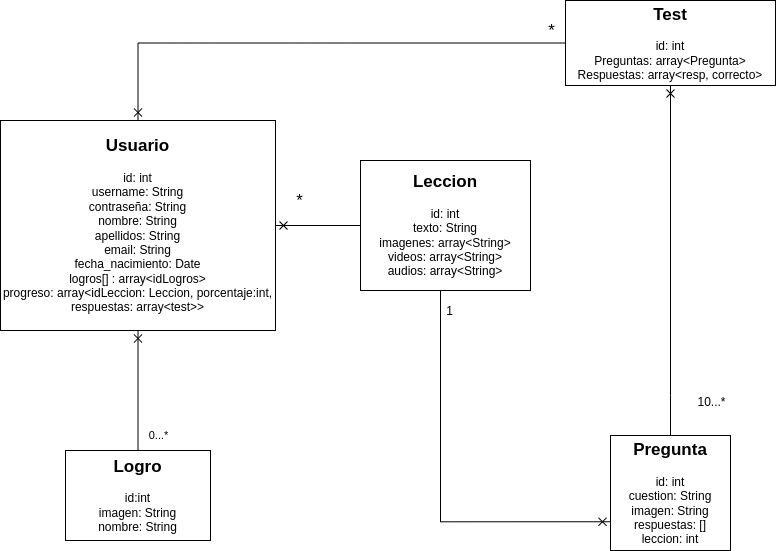
\includegraphics[width=1\textwidth]{imagenes/c5/diagramadeclases.png}}
    \caption{Diagrama de clases de nuestro proyecto donde se muestran las relaciones entre las diferentes clases que componen el sistema.}
    \label{fig:diagramadeclases}    
\end{figure}

Como se puede observar, disponemos de cinco clases principales: Usuario, Lección, Test, Pregunta y Logro. Estas entidades se han relacionado siguiendo 
la descripción del sistema que se ha realizado hasta ahora.